\begin{frame}{}
    \centering
        \Huge\bfseries
    \textcolor{yellow}{Deleted Scenes}
\end{frame}

\begin{frame}{Notable Individuals in the V8 0-day Research Community}
    \begin{itemize}
        \item Samuel Gro$\beta$ -- Head of V8 Security Team, former Google Project Zero
        \item Clement Lecigne -- Google Threat Analysis Group, who has ``burned" many 0-days in V8 
        \item Hossein Lotfi -- Zero-day Initiative, amazing documentation about V8 from Pwn2Own 
        \item Man Yue Mo -- GitHub Security Lab, great writeups about 0-day Vulnerabilities 
        \item Zhenghang Xiao -- Independent Security Researcher speaking at Black Hat 2023
        \item Alisa Esage -- Independent Security Researcher with great YouTube talk
    \end{itemize}
    \break
    \href{https://phrack.org/issues/70/3.html}{\color{pink}{Samuel Grob's phrack.org article on V8 exploitation}}
    \break
    \href{https://www.youtube.com/watch?v=WouAptHlyC4}{\color{pink}{Alisa Esage's Modern Attacks on Google Chrome YouTube talk}}
\end{frame}

\begin{frame}{Type Confusion in Value Serializer -- CVE-2023-1214}{Discovered by Man Yue Mo of GitHub Security Lab}
    \begin{columns}
        \begin{column}{0.7\textwidth}
            \begin{itemize}
                \item This vulnerability involves incorrect assumptions made during a Map (HiddenClass) transition.
                \item Many objects in JavaScript are likely to be the same, so V8 saves on memory by re-using object mappings.
                \item Maps will point to other maps, forming a tree.
                \item Map transitions occur when new properties are added or removed from objects creating a ``never-before-seen" layout. 
            \end{itemize}
        \href{https://bugs.chromium.org/p/chromium/issues/detail?id=1412487}{\color{pink}{crbug-1412487}}
        \end{column}
        \begin{column}{0.3\textwidth}
            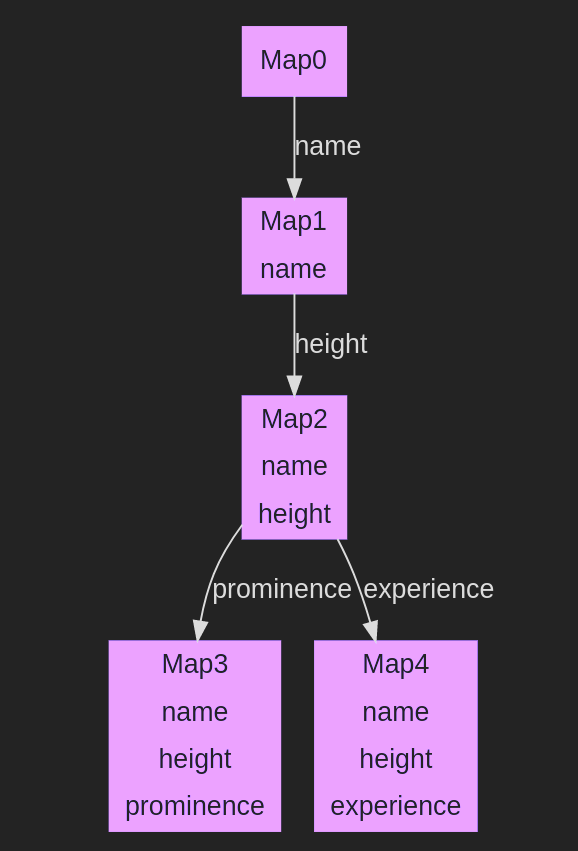
\includegraphics[height=6.5cm]{images/v8-hiddenclass.png}
        \end{column}
    \end{columns}
\end{frame}

\begin{frame}[fragile]{Type Confusion Example}
    \begin{columns}
        \begin{column}{0.5\textwidth}
            \usemintedstyle{vim}
            \inputminted{C}{code/type-confusion.tex}
        \end{column}
        \begin{column}{0.5\textwidth}
            \usemintedstyle{vim}
            \inputminted{C}{code/type-confusion-exploit.tex}
        \end{column}
    \end{columns}
\end{frame}